% ============================================================
%   EPSS-TPG end-to-end model architecture
% ============================================================
%
% Single-file, standalone TikZ diagram covering the full pipeline:
%   1. Raw CVE text input
%   2. spaCy linguistic frontend (tokens, NER, dependencies, chunks)
%   3. How nodes and edges are linked (13 base edge types)
%   4. Security frontend: regex + curated dictionaries
%   5. SecBERT contextual embeddings joined to spaCy nodes
%      (WordPiece subtoken pooling, character-span alignment)
%   6. PyG tensor construction (node features, edge_index, edge_type)
%   7. Multi-view GGNN backbone + node-conditioned attention fusion
%   8. Mean+max pooling, tabular branch, fusion head, sigmoid output
%
% Verified against the source (2026-05-15):
%   tpg/frontends/spacy_frontend.py        steps 1..5 of TPG construction
%   tpg/frontends/security_frontend.py     regex + keyword extractors
%   tpg/passes/security_relations.py       10 SEC_* edge types
%   tpg/frontends/hybrid_security_frontend.py  SecBERT WordPiece pooling
%   tpg/exporters/exporters.py             781-dim node features (13 + 768)
%   epss/tabular_features.py               55-dim tabular vector
%   epss/edge_aware_layers.py              ViewEncoder + ViewAttentionFusion
%   epss/gnn_model.py                      HybridEPSSClassifier head
%
% Compile:
%   pdflatex -interaction=nonstopmode model_architecture.tex
% ============================================================

\documentclass[10pt]{article}

\usepackage[a2paper, portrait, margin=12mm]{geometry}
\usepackage{tikz}
\usepackage{amsmath}
\usepackage{amssymb}
\pagestyle{empty}

\usetikzlibrary{positioning, arrows.meta, calc, fit, backgrounds, shapes.geometric, shapes.multipart}

% -- Colour palette (printer-friendly, distinguishable in grayscale) --
\definecolor{stageA}{RGB}{236,244,255}     % light blue  (text input)
\definecolor{stageB}{RGB}{223,239,223}     % light green (spaCy)
\definecolor{stageC}{RGB}{255,236,217}     % light orange (security pass)
\definecolor{stageD}{RGB}{240,228,247}     % light purple (SecBERT)
\definecolor{stageE}{RGB}{255,247,210}     % light yellow (PyG tensors)
\definecolor{stageF}{RGB}{217,237,237}     % light teal  (multi-view GNN)
\definecolor{stageG}{RGB}{255,222,222}     % light pink  (tabular branch)
\definecolor{stageH}{RGB}{229,229,229}     % light grey  (head + output)

\definecolor{nodeBase}{RGB}{ 70,130,180}
\definecolor{nodeSec}{RGB}{200, 80, 80}
\definecolor{edgeBase}{RGB}{ 60, 60, 60}
\definecolor{edgeSec}{RGB}{160, 50, 50}
\definecolor{accent}{RGB}{ 20, 70,140}

% -- Text-mode helper macros (used inside node text) --
\newcommand{\detail}[1]{{\scriptsize #1}}
\newcommand{\tinydet}[1]{{\tiny #1}}

% -- Common tikz styles --
\tikzset{
    stage/.style={
        rounded corners=2pt, draw=black!50, line width=0.4pt,
        inner sep=6pt, align=left,
        font=\footnotesize
    },
    title/.style={font=\sffamily\bfseries\footnotesize, text=accent},
    detailnode/.style={font=\scriptsize},
    tinydetnode/.style={font=\tiny},
    bignode/.style={
        rounded corners=2pt, draw=nodeBase, fill=white, line width=0.4pt,
        inner sep=2.5pt, font=\tiny\sffamily, minimum height=4mm
    },
    secnode/.style={
        rounded corners=2pt, draw=nodeSec, fill=white, line width=0.4pt,
        inner sep=2.5pt, font=\tiny\sffamily, minimum height=4mm
    },
    flow/.style={-{Stealth[length=2.5mm]}, line width=0.55pt, draw=black!75},
    sec/.style ={-{Stealth[length=2mm]},  line width=0.45pt, draw=edgeSec, dashed},
    lin/.style ={-{Stealth[length=2mm]},  line width=0.4pt,  draw=edgeBase}
}

\begin{document}

\begin{tikzpicture}[node distance=10mm and 14mm]

% ============================================================
%  STAGE 1: INPUT
% ============================================================
\node[stage, fill=stageA, text width=64mm] (input) {
    \textbf{1.\ Raw CVE record} \\[2pt]
    \detail{Description text plus, optionally, one or more LLM
    summary columns. Source-CSV format (Sec4AI4Aec, Megavul) or
    NVD JSON.}\\[1pt]
    \tinydet{Example: \texttt{"A buffer overflow in OpenSSL 1.0.1f
    allows a remote attacker to ..."}}
};

% ============================================================
%  STAGE 2: spaCy frontend
% ============================================================
\node[stage, fill=stageB, text width=85mm, below=of input] (spacy) {
    \textbf{2.\ spaCy linguistic frontend}
    \hfill \tinydet{\texttt{en\_core\_web\_sm}}\\[2pt]
    \detail{Five-step build, one paragraph at a time:}
    \begin{itemize}\setlength\itemsep{0pt}\setlength\topsep{1pt}
        \item[\textbullet] tokenise + POS-tag + lemmatise + dependency-parse
        \item[\textbullet] named-entity recognition (PERSON, ORG, GPE, $\ldots$)
        \item[\textbullet] sentence segmentation
        \item[\textbullet] noun-chunk detection
        \item[\textbullet] character offsets preserved per token
    \end{itemize}
};

% ============================================================
%  STAGE 3: TPG construction (nodes + 13 base edges)
% ============================================================
\node[stage, fill=stageB, text width=95mm, below=of spacy] (tpg) {
    \textbf{3.\ TPG construction: 13 node types, 13 base edge types}\\[2pt]
    \detail{One DOCUMENT root. For each paragraph: one PARAGRAPH node,
    each sentence becomes a SENTENCE, each spaCy token becomes a TOKEN.
    Spans become ENTITY / NOUN\_PHRASE / VERB\_PHRASE / CLAUSE nodes;
    content verbs become PREDICATE nodes; their dependents become
    ARGUMENT nodes with SRL roles inferred from the dep label.}\\[3pt]
    \detail{Edges are wired as the nodes are created:}\\[1pt]
    \tinydet{CONTAINS}\hfill\tinydet{DOC$\to$PARA$\to$SENT$\to$\{TOKEN, ENTITY, NP, VP, CLAUSE, PRED\}}\\
    \tinydet{BELONGS\_TO}\hfill\tinydet{ENTITY/NP/VP/CLAUSE/PRED/ARG $\to$ TOKEN}\\
    \tinydet{DEP}\hfill\tinydet{TOKEN (head) $\to$ TOKEN (child), dep label stored on edge}\\
    \tinydet{NEXT\_TOKEN}\hfill\tinydet{adjacent TOKEN$\to$TOKEN, intra and inter sentence}\\
    \tinydet{NEXT\_SENT}\hfill\tinydet{adjacent SENT$\to$SENT (document order)}\\
    \tinydet{NEXT\_PARA}\hfill\tinydet{adjacent PARA$\to$PARA}\\
    \tinydet{SRL\_ARG}\hfill\tinydet{TOKEN/ARG $\to$ PRED, role label (ARG0, ARG1, ARGM-*)}\\
    \tinydet{COREF, RST\_RELATION, DISCOURSE,}\hfill\tinydet{added later by enrichment passes}\\
    \tinydet{ENTITY\_REL, SIMILARITY, AMR\_EDGE}\hfill\tinydet{(CoreferencePass, DiscoursePass, $\ldots$)}
};

% ============================================================
%  Mini example TPG (alongside stage 3)
% ============================================================
\node[stage, fill=white, text width=58mm, right=14mm of tpg, draw=black!40] (example) {
    \textbf{Example sub-graph}\\[2pt]
    \detail{For \texttt{"Buffer overflow in OpenSSL 1.0.1f"}}
    \\[6mm]
    \begin{tikzpicture}[remember picture, scale=0.95]
      \node[bignode] (S)  at (0,1.6) {SENTENCE};
      \node[bignode] (T1) at (-1.7,0.3) {TOKEN: Buffer};
      \node[bignode] (T2) at (-0.6,0.3) {TOKEN: overflow};
      \node[bignode] (T3) at (0.5,0.3) {TOKEN: in};
      \node[bignode] (T4) at (1.6,0.3) {TOKEN: OpenSSL};
      \node[bignode] (NP) at (-1.2,-0.9) {NOUN\_PHRASE: Buffer overflow};
      \node[bignode] (E)  at (1.7,-0.9) {ENTITY: OpenSSL};
      \draw[lin] (S) -- node[tinydetnode, midway, sloped, above, yshift=-2pt] {CONTAINS} (T1);
      \draw[lin] (S) -- (T2);  \draw[lin] (S) -- (T3);  \draw[lin] (S) -- (T4);
      \draw[lin] (S) -- (NP);
      \draw[lin] (NP) -- node[tinydetnode, sloped, midway, above, yshift=-2pt] {BELONGS\_TO} (T1);
      \draw[lin] (NP) -- (T2);
      \draw[lin] (E)  -- (T4);
      \draw[lin] (T1) to[bend right=12] node[tinydetnode, midway, below] {NEXT\_TOKEN} (T2);
      \draw[lin] (T2) to[bend right=12] (T3);
      \draw[lin] (T3) to[bend right=12] (T4);
    \end{tikzpicture}
};

% ============================================================
%  STAGE 4: Security pass (regex + dict + 10 SEC_* edges)
% ============================================================
\node[stage, fill=stageC, text width=95mm, below=14mm of tpg] (sec) {
    \textbf{4.\ Security frontend: regex + curated dictionaries}\\[2pt]
    \detail{Adds 12 security node types on top of the linguistic
    graph (frontend), then 10 typed SEC\_* edges (SecurityRelationsPass).}
    \\[3pt]
    \detail{Rule sources:}\\
    \tinydet{\texttt{CVE-\textbackslash d\{4\}-\textbackslash d\{4,\}}}\hfill\tinydet{$\to$ ENTITY tagged CVE\_ID}\\
    \tinydet{\texttt{CWE-\textbackslash d\{1,4\}}}\hfill\tinydet{$\to$ ENTITY tagged CWE\_ID}\\
    \tinydet{\texttt{\textbackslash b\textbackslash d+\textbackslash .\textbackslash d+(\textbackslash .\textbackslash d+)*\textbackslash b}}\hfill\tinydet{$\to$ ENTITY tagged VERSION (CVSS scores filtered)}\\
    \tinydet{\texttt{CVSS:3\textbackslash .\textbackslash d/...}}\hfill\tinydet{$\to$ ENTITY tagged SEVERITY}\\
    \tinydet{C-style function regex}\hfill\tinydet{$\to$ ENTITY tagged CODE\_ELEMENT}\\
    \tinydet{\textsc{software} dictionary ($\sim$300 names)}\hfill\tinydet{$\to$ ENTITY tagged SOFTWARE}\\
    \tinydet{\textsc{attack vector} dict}\hfill\tinydet{$\to$ ENTITY tagged ATTACK\_VECTOR}\\
    \tinydet{\textsc{impact} dict (rce, dos, escalation, ...)}\hfill\tinydet{$\to$ ENTITY tagged IMPACT}\\
    \tinydet{\textsc{vuln type} dict (overflow, XSS, ...)}\hfill\tinydet{$\to$ ENTITY tagged VULN\_TYPE}\\
    \tinydet{\textsc{remediation} regex set}\hfill\tinydet{$\to$ ENTITY tagged REMEDIATION}
    \\[4pt]
    \detail{SecurityRelationsPass then emits cartesian-product edges:}\\
    \tinydet{\texttt{SEC\_AFFECTS}\,(CVE$\to$SW),\;
                \texttt{SEC\_HAS\_VERSION}\,(SW$\to$VER),\;
                \texttt{SEC\_CLASSIFIED\_AS}\,(CVE$\to$CWE),}\\
    \tinydet{\texttt{SEC\_LOCATED\_IN}\,(VULN$\to$CODE),\;
                \texttt{SEC\_EXPLOITED\_BY}\,(CVE$\to$AV),\;
                \texttt{SEC\_CAUSES}\,(AV$\to$IMPACT),}\\
    \tinydet{\texttt{SEC\_MITIGATED\_BY}\,(CVE$\to$REM),\;
                \texttt{SEC\_USES\_FUNCTION}\,(CVE$\to$CODE),\;
                \texttt{SEC\_THREATENS}\,(AV$\to$SW),}\\
    \tinydet{\texttt{SEC\_HAS\_SEVERITY}\,(CVE$\to$SEV).
                Active only when \texttt{-{}-include-security-edges} is on;
                edge-type vocabulary then grows from 13 to 23.}
};

% ============================================================
%  STAGE 5: SecBERT embedding pass
% ============================================================
\node[stage, fill=stageD, text width=95mm, below=10mm of sec] (sbert) {
    \textbf{5.\ SecBERT embedding pass joins to spaCy nodes}
    \hfill \tinydet{\texttt{jackaduma/SecBERT}, frozen, 768-dim}\\[3pt]
    \detail{Three encodings, all from the same SecBERT forward pass:}\\[1pt]
    \tinydet{(a)} \detail{SENTENCE nodes get the [CLS] embedding of the sentence text.}\\
    \tinydet{(b)} \detail{TOKEN nodes get the \textbf{character-span-aligned} mean of WordPiece subtoken vectors.}\\
    \tinydet{(c)} \detail{ENTITY and NOUN\_PHRASE nodes get a [CLS] embedding of their text (if not already set).}
    \\[3pt]
    \detail{Alignment between WordPiece subtokens and spaCy tokens:}\\[1pt]
    \tinydet{1.\ SecBERT tokenises sentence text with \texttt{return\_offsets\_mapping=True}.}\\
    \tinydet{2.\ For each spaCy TOKEN node, find the subtoken indices whose char span overlaps the token's char span.}\\
    \tinydet{3.\ \texttt{aligned = subword\_embeds[matching].mean(dim=0)}, stored at \texttt{node.properties.extra["embedding"]}.}\\
    \tinydet{4.\ Nodes without text get the zero vector.}
};

% ============================================================
%  STAGE 6: PyG tensor build
% ============================================================
\node[stage, fill=stageE, text width=95mm, below=10mm of sbert] (pyg) {
    \textbf{6.\ PyG tensor construction (per CVE graph)}\\[2pt]
    \detail{The exporter walks the TPG once and produces:}\\[1pt]
    \tinydet{\texttt{x}\ \ \ : $N\times 781$}\hfill
    \tinydet{$=$ \,[node-type one-hot (13)] $\Vert$ [SecBERT 768-dim]\,
              (784 with \texttt{-{}-add-source-labels})}\\
    \tinydet{\texttt{edge\_index}\,: $2\times M$}\hfill
    \tinydet{source$\to$target indices over all kept edges}\\
    \tinydet{\texttt{edge\_type}\,\;: $M$}\hfill
    \tinydet{integer in $[0, R)$ where $R=13$ or $R=23$ (base $+$ SEC\_*)}\\
    \tinydet{\texttt{edge\_attr}\,\;: $M\times R$}\hfill
    \tinydet{one-hot of \texttt{edge\_type}}\\
    \tinydet{\texttt{y}\,\;\;\;\;\;\;\;: scalar}\hfill
    \tinydet{soft EPSS in $[0,1]$ \textbf{or} binary KEV label}\\
    \tinydet{\texttt{tabular}: 55-dim or 57-dim}\hfill
    \tinydet{built only when \texttt{-{}-hybrid} is set}
};

% ============================================================
%  STAGE 7: Multi-view GNN backbone + fusion
% ============================================================
\node[stage, fill=stageF, text width=95mm, below=12mm of pyg] (mv) {
    \textbf{7.\ Multi-view GGNN with node-conditioned attention fusion}\\[3pt]
    \detail{Input projection $H^{(0)} = \mathrm{Dropout}(\mathrm{GELU}(\mathrm{LayerNorm}(W_{\text{in}}\,X)))$\,,
    $H^{(0)}\in\mathbb{R}^{N\times h}$, $h=128$.}\\[3pt]
    \detail{Edges are partitioned into $V$ views:}\\
    \tinydet{syntactic}\hfill\tinydet{DEP, CONTAINS, BELONGS\_TO}\\
    \tinydet{sequential}\hfill\tinydet{NEXT\_TOKEN, NEXT\_SENT, NEXT\_PARA}\\
    \tinydet{semantic}\hfill\tinydet{COREF, SRL\_ARG, AMR\_EDGE}\\
    \tinydet{discourse}\hfill\tinydet{RST\_RELATION, DISCOURSE, ENTITY\_REL, SIMILARITY}\\
    \tinydet{security}\hfill\tinydet{all SEC\_* (only when security edges are enabled)}
    \\[3pt]
    \detail{Per view, a Gated Graph Neural Network (Li et al., 2015):
    $H_v = \mathrm{ViewEncoder}_v(H^{(0)}, E_v)$ runs $K\!=\!3$ message-passing
    steps over that view's edges, with a residual, LayerNorm and Dropout.}
    \\[3pt]
    \detail{Node-conditioned fusion (per node $i$):
    a query $q_i$ from $H^{(0)}_i$ and per-view keys $k_i^v$ from $H_v[i,:]$
    produce scaled-dot-product scores $q_i\!\cdot k_i^v/\sqrt{h}$;
    softmax over $V$ gives weights $\alpha_i^v$; the fused embedding is
    $h_i = \sum_v \alpha_i^v\, H_v[i,:]$.}
};

% Mini schematic of the multi-view backbone, sitting alongside.
\node[stage, fill=white, text width=58mm, right=14mm of mv, draw=black!40] (mvfig) {
    \textbf{Multi-view backbone}\\[2pt]
    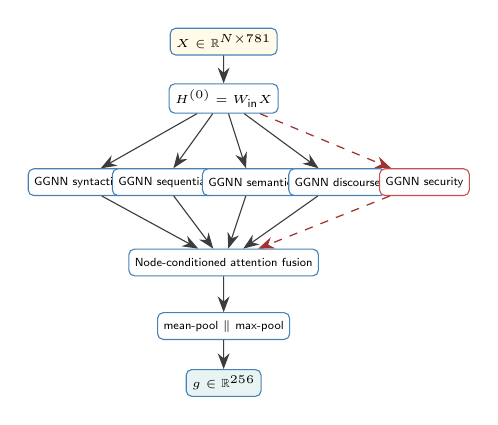
\begin{tikzpicture}[scale=0.85, transform shape]
      \node[bignode, fill=stageE!50] (X) at (0,2.4) {$X \in \mathbb{R}^{N\times 781}$};
      \node[bignode] (H0) at (0,1.55) {$H^{(0)} = W_{\text{in}} X$};
      \node[bignode] (V1) at (-2.2,0.3) {GGNN syntactic};
      \node[bignode] (V2) at (-0.9,0.3) {GGNN sequential};
      \node[bignode] (V3) at (0.4,0.3)  {GGNN semantic};
      \node[bignode] (V4) at (1.7,0.3)  {GGNN discourse};
      \node[secnode] (V5) at (3.0,0.3)  {GGNN security};
      \node[bignode] (F)  at (0,-0.9) {Node-conditioned attention fusion};
      \node[bignode] (P)  at (0,-1.85) {mean-pool $\Vert$ max-pool};
      \node[bignode, fill=stageF!60] (G) at (0,-2.7) {$g \in \mathbb{R}^{256}$};
      \draw[lin] (X) -- (H0);
      \draw[lin] (H0) -- (V1); \draw[lin] (H0) -- (V2);
      \draw[lin] (H0) -- (V3); \draw[lin] (H0) -- (V4);
      \draw[sec] (H0) -- (V5);
      \draw[lin] (V1) -- (F); \draw[lin] (V2) -- (F);
      \draw[lin] (V3) -- (F); \draw[lin] (V4) -- (F);
      \draw[sec] (V5) -- (F);
      \draw[lin] (F) -- (P);
      \draw[lin] (P) -- (G);
    \end{tikzpicture}
    \\
    \tinydet{Solid = always on. Dashed red = security view, active only
    with \texttt{-{}-include-security-edges}.}
};

% ============================================================
%  STAGE 8: Tabular branch
% ============================================================
\node[stage, fill=stageG, text width=95mm, below=12mm of mv] (tab) {
    \textbf{8.\ Tabular branch (hybrid mode only)}\\[3pt]
    \detail{Per-CVE feature vector \texttt{tabular} (55-dim default,
    57 when EPSS is kept as input):}\\
    \tinydet{$\bullet$ CVSS v3 score (1) + has-CVSS flag (1)}\\
    \tinydet{$\bullet$ CVSS v3 vector components (4+2+3+2+2+3+3+3 = 22 one-hot)}\\
    \tinydet{$\bullet$ Top-25 CWE multi-hot + ``other'' bucket (26)}\\
    \tinydet{$\bullet$ CWE count, references count, vulnerability age, public-exploit
              flag, exploit count (1 each)}\\
    \tinydet{$\bullet$ EPSS score, EPSS percentile (optional, +2)}
    \\[3pt]
    \detail{Tabular MLP:
    $\mathrm{Linear}(\textsc{tab}, 128) \to \mathrm{BN} \to \mathrm{ReLU} \to \mathrm{Drop}
    \to \mathrm{Linear}(128, 64) \to \mathrm{ReLU} \to \mathrm{Drop}$.}\\
    \detail{Output: $t \in \mathbb{R}^{64}$.}
};

% ============================================================
%  STAGE 9: Fusion head and prediction
% ============================================================
\node[stage, fill=stageH, text width=95mm, below=10mm of tab] (head) {
    \textbf{9.\ Fusion head and prediction}\\[3pt]
    \detail{Inputs: graph vector $g\in\mathbb{R}^{256}$ from stage 7
    and tabular embedding $t\in\mathbb{R}^{64}$ from stage 8.}\\[2pt]
    \detail{Concatenate, then a 3-layer MLP with batch norm and dropout
    in the middle:}\\[1pt]
    \tinydet{$[g; t]\in\mathbb{R}^{320}$
        $\to$ Linear(320, 128) $\to$ BN $\to$ ReLU $\to$ Drop
        $\to$ Linear(128, 64) $\to$ ReLU $\to$ Drop
        $\to$ Linear(64, 1)}
    \\[2pt]
    \detail{Output logit $\hat\ell\in\mathbb{R}$; predicted probability $\hat p = \sigma(\hat\ell)\in[0,1]$.}\\[3pt]
    \detail{Training:
    BCE-with-logits against the label $y$,
    with a positive-class weight $w^+ =$ negatives/positives so the rare
    high-EPSS / KEV class is not drowned out.
    Optimiser: AdamW, lr $=10^{-3}$, weight decay $=10^{-4}$, grad clip 1.0.
    ReduceLROnPlateau on val PR-AUC, early stop after 15 epochs without gain.}\\[3pt]
    \detail{Inference: $\hat p$ is the predicted exploitation probability;
    risk tier (LOW/MEDIUM/HIGH/CRITICAL) is read off the operational
    thresholds 0.1, 0.4, 0.7.}
};

% ============================================================
%  Vertical flow arrows down the main column
% ============================================================
\draw[flow] (input) -- (spacy);
\draw[flow] (spacy) -- (tpg);
\draw[flow] (tpg)   -- (sec);
\draw[flow] (sec)   -- (sbert);
\draw[flow] (sbert) -- (pyg);
\draw[flow] (pyg)   -- (mv);
\draw[flow] (mv)    -- (tab);
\draw[flow] (tab)   -- (head);

% Side annotations
\draw[lin, dashed] (tpg.east) -- node[tinydetnode, midway, above, sloped] {feeds} (example.west);
\draw[lin, dashed] (mv.east)  -- node[tinydetnode, midway, above, sloped] {detailed view} (mvfig.west);

% Title
\node[font=\sffamily\large\bfseries, above=4mm of input, text=accent]
    {EPSS-TPG: end-to-end model architecture};

\end{tikzpicture}

\end{document}
